\documentclass[11pt]{article}

% Any percent sign marks a comment to the end of the line

% Every latex document starts with a documentclass declaration like this
% The option dvips allows for graphics, 12pt is the font size, and article
%   is the style

\usepackage[pdftex]{graphicx}
\usepackage{url}

\usepackage{soul}

\usepackage{hyperref} % Using hyperlink

\usepackage{graphicx} % Required for including images

\usepackage{setspace}
\setstretch{1}


%\usepackage{geometry}
% \geometry{
% left=7.6cm,top=0.1cm,right=1cm,bottom=0.1cm,nohead,nofoot
% }

% These are additional packages for "pdflatex", graphics, and to include
% hyperlinks inside a document.

\setlength{\oddsidemargin}{-0.25in}
\setlength{\textwidth}{7in}
\setlength{\topmargin}{-0.8in}
\setlength{\textheight}{9.2in}

% These force using more of the margins that is the default style

\begin{document}

% Everything after this becomes content
% Replace the text between curly brackets with your own

%\title{Hong Kong Labour Market Data Visualization}
%\author{Fong Chun Him (3035377115), Wu Szu Han (3035562617)}
%\date{November 17, 2020}

% You can leave out "date" and it will be added automatically for today
% You can change the "\today" date to any text you like


%\maketitle

% This command causes the title to be created in the document

\begin{center}
\Huge{EGuard Documentation on Technologies Used}
\end{center}

\section*{\large{1 \hspace{10pt} Overview}}
EGuard is a scam detection solution which alerts users to possible scams. At the current stage, a warning banner has been developed to alert users to unrecognized email sender addresses. \\
\\
Mailu is used in EGuard's prototype as the mail server since Mailu is open source, easy-to-install and full-featured. A Linux machine is used to host the mail server since Linux is open source, flexible, secure and reliable for running servers.

\begin{center}
	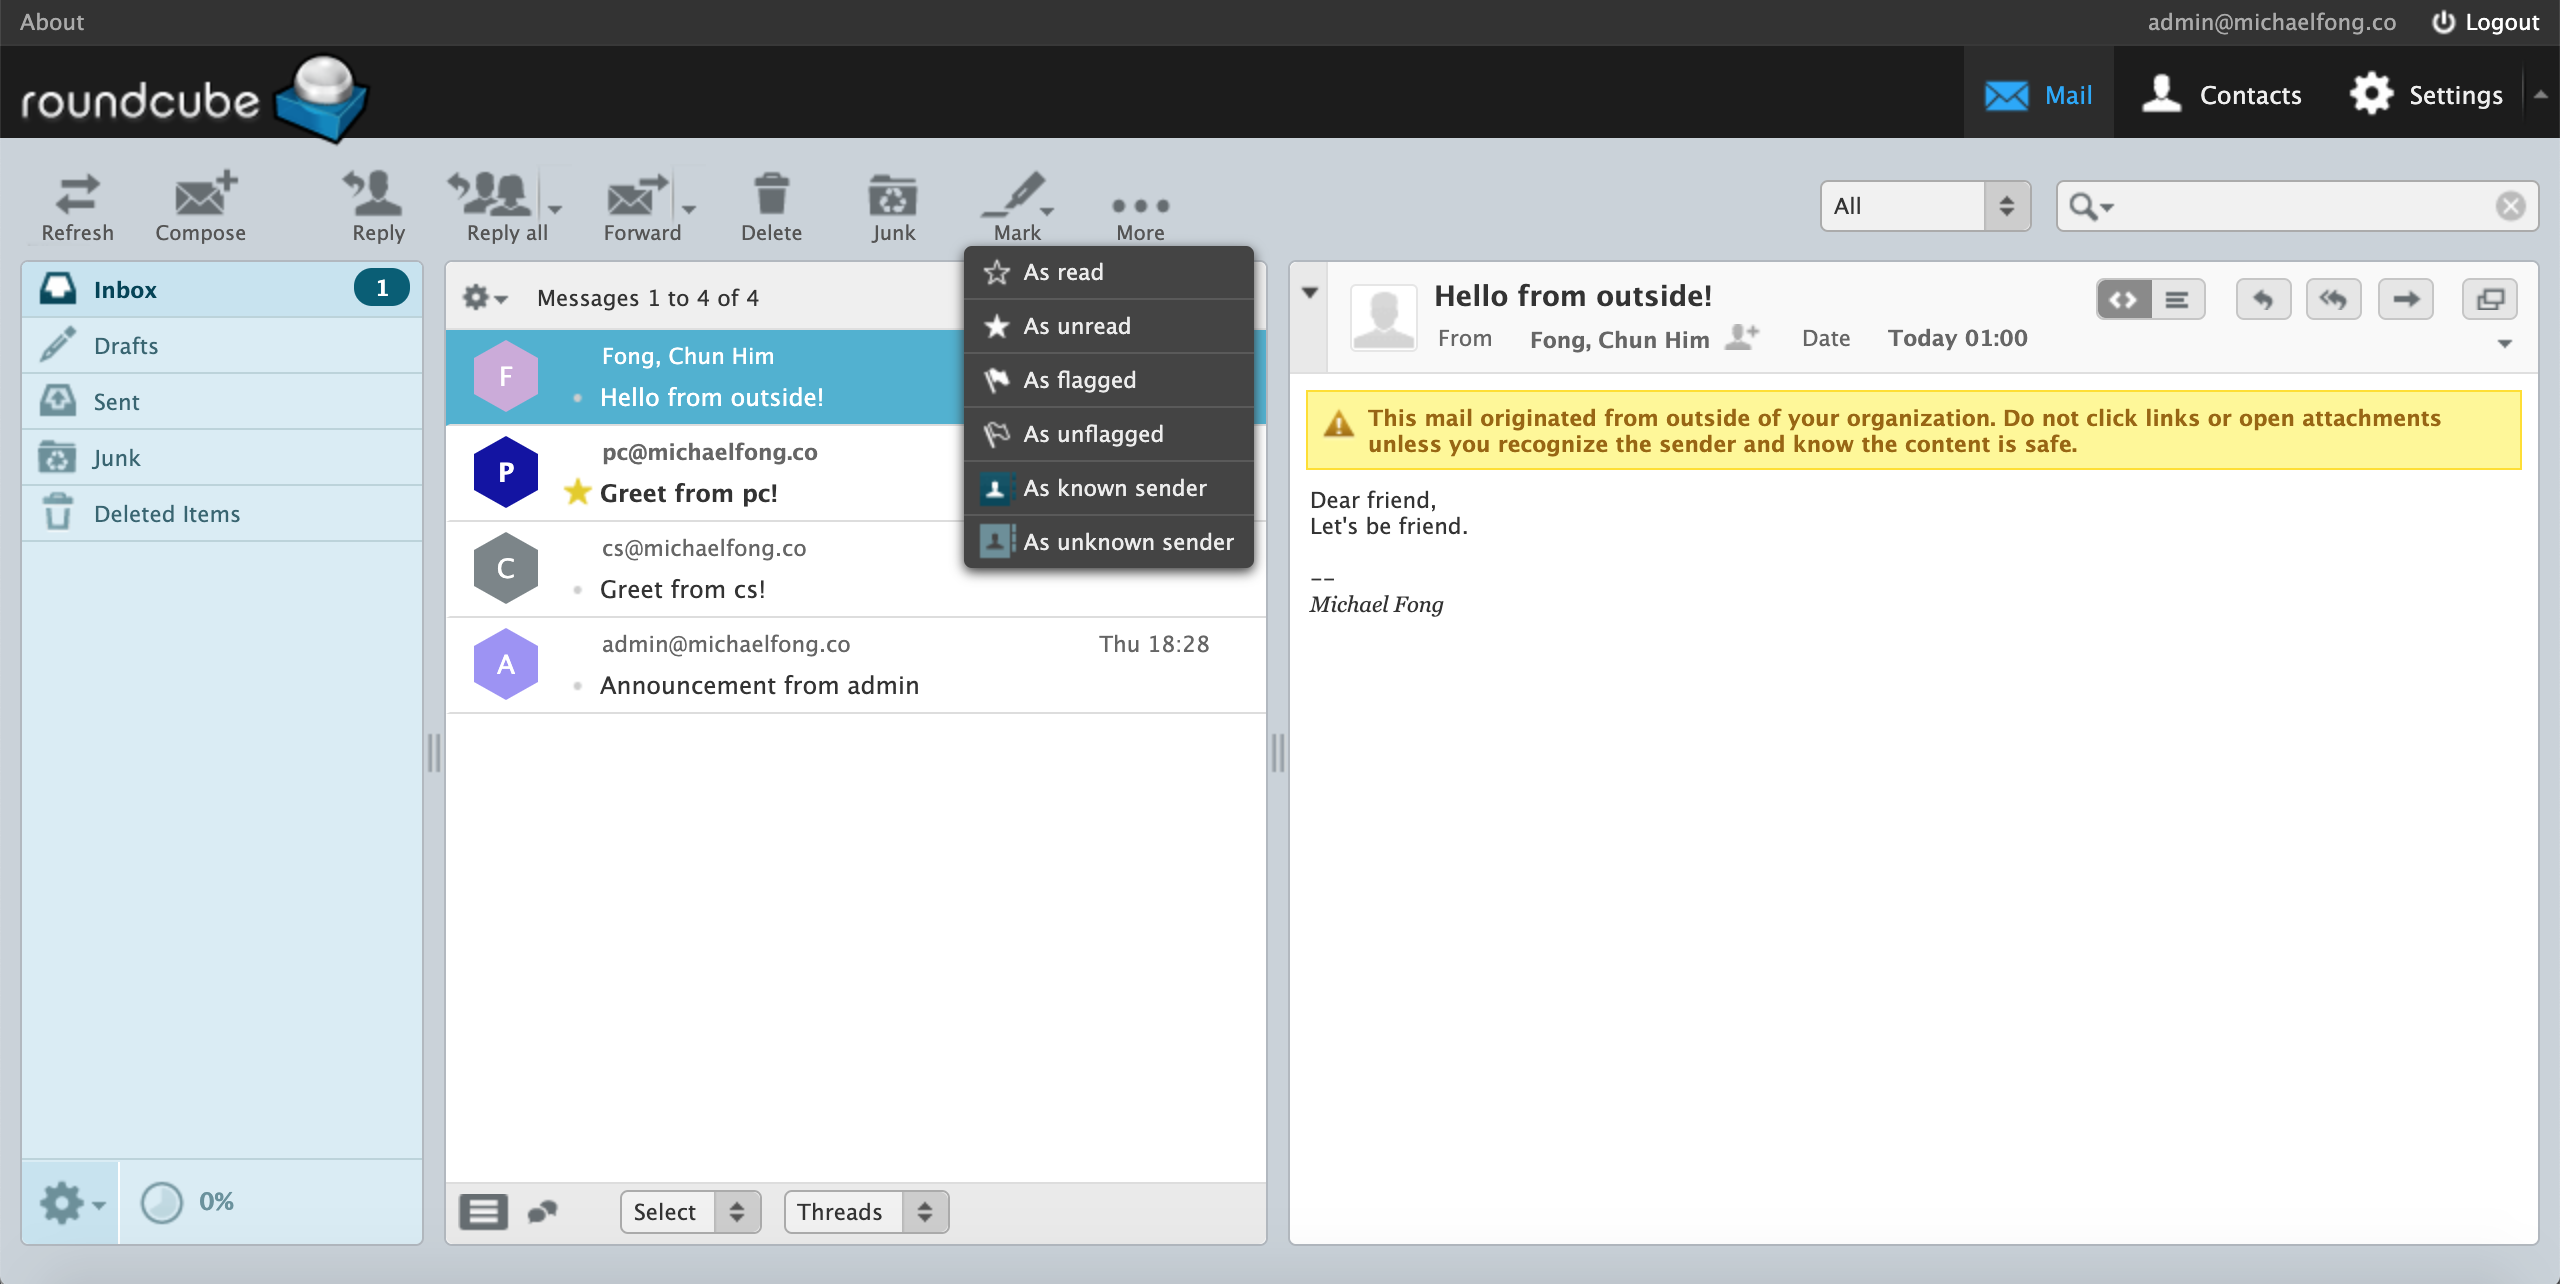
\includegraphics[width=1\columnwidth]{roundcube} % Example image
\end{center}

\noindent{Live demo: \href{https://mail.michaelfong.co}{https://mail.michaelfong.co}}

\section*{\large{2 \hspace{10pt} Architecture}}
\subsection*{2.1 \hspace{10pt} Mailu}
Mailu version 1.7, which is an open source mail server as a set of Docker images, is installed in a Linux machine. Mailu uses postfix as the mail transfer agent (MTA) and is configured to use Roundcube as the webmail. Mailu contains other microservices such as a proxy server and a web administration interface and has security features such as enforced TLS and anti-spoofing.

\subsection*{2.2 \hspace{10pt} Mail Transfer Agent}
Using postfix as the MTA is not a must. Choice of the MTA does not matter much to the scam detection utility being developed. The MTA can be replaced by other MTAs such as exim and sendmail if Mailu is not used as clients' mail server. 

\subsection*{2.3 \hspace{10pt} Webmail}
A webmail is a web-based service that allows users to access their emails. Interfaces have to be developed for each choice of the webmail. In EGuard's prototype, Roundcube is used. Roundcube plugins are written in php and javascript and installed by adding a folder inside the Roundcube plugin directory. A warning banner is developed to display a warning message at the beginning of the email content whenever an email sender is not recognized before. Menu buttons are developed to recognize or unrecognize email senders of selected emails. A recognized email sender list is persistently stored inside the linux machine which hosts the mail server. gRPC is used as the protocol for webmail to communicate with the EGuard backend to query or update the recognized email sender list. Whether a warning banner displays or not depends on the query result. It is possible for the EGuard backend and the recognized email sender list to be stored in another linux machine.

\section*{\large{3 \hspace{10pt} Implementations}}

\subsection*{3.1 \hspace{10pt} Docker and Docker Compose}
Docker deployment ensures compatibility, consistency and easy upgrades of the EGuard mail system.
\begin{itemize}

\item Compatibility: The EGuard mail system works on any linux machines that support Docker. No other packages or installation are required other than pulling the set of EGuard docker images and running the docker containers. There are no worries that EGuard requires packages unsupported by the host machine.

\item Consistency: Each docker container is an isolated environment. There are no dependency conflicts between the application inside a container and applications outside the container. Misconfiguration is avoided since the entire environment is set up consistently and automatically by running the set of pre-configured docker images. All host machines run the EGuard mail system with the same configurations by default. A utility is being developed for users to generate their own configurations.

\item Easy upgrades: When a new version of the EGuard mail system is available, changes are committed to the docker images and pushed to remote repositories. Users can upgrade and downgrade their docker images freely without losing their emails and data as emails and user data are persistently stored in their linux machine outside the docker containers.

\end{itemize}

\noindent{Docker compose further automates the process of creating, starting and stoping the various containers. Docker network creation, volume mounting and port publishing are pre-configured.}


\subsection*{3.2 \hspace{10pt} Linux Machine}
EGuard mail server is hosted on the user's linux machine, which persistently stores user emails and data and serves the EGuard backend which is being developed. At the first stage of development, a pickle file is reserved for each email account to hold a set of recognized email sender addresses (in binary format for performance). This pickle file is stored inside the user account directory in the linux machine. A gRPC python server keeps running to accept queries from the Roundcube webmail client about the set of recognized email sender addresses and accept updates on the set. gRPC is used as the communication protocol because it has lower latency and higher throughput than REST and websocket due to the use of HTTP/2 for transport and protobuf as a more lightweight data format. Python is used for both gRPC server and gRPC client because of the use of virtual environment and the ease of scripting.

\subsection*{3.3 \hspace{10pt} Roundcube Plugin}
Roundcube is an open source webmail client, where plugins can be developed in php and javascript and installed. There is an existing plugin that displays a warning banner if an email sender address does not match a customizable regular expression. Nonetheless, it is not implemented to communicate with a list of recognized sender addresses stored outside of Roundcube and there is no way to update the list on-the-fly inside Roundcube. Therefore, a plugin is being developed on top of the warning banner plugin to implement the client-server communication between Roundcube and the linux machine and implement the user interfaces.

\section*{\large{4 \hspace{10pt} Variations}}
Mailu acts as a backbone of the EGuard mail system for the prototype being developed. Nonetheless, components of Mailu can be replaced by other services independently. Minimally, EGuard can be deployed to existing mail systems as a collection of add-ons, including Roundcube plugins and the EGuard backend for email analysis and scam detection. For mail system that uses email clients other than Roundcube, either the users are encouraged to switch to Roundcube, or new plugins are developed for other email clients to implement the same functions. For users willing to set up a mail system from scratch, either they can use the current Mailu architecture, or a new architecture is assembled based on their needs. Besides, the EGuard backend for email analysis and scam detection is not necessarily deployed in the linux machine hosting the mail server but can also be deployed in another machine as long as a gRPC server can be run. \\
\\
At a future stage, more sophisticated email analysis can be done in the EGuard backend. gRPC allows email clients to send emails to the backend for analysis and receive responses.

%\section*{\large{5 \hspace{10pt} References}}
%\noindent{[1] \href{https://ijcsit.com/docs/Volume\%207/vol7issue5/ijcsit20160705014.pdf}{https://ijcsit.com/docs/Volume\%207/vol7issue5/ijcsit20160705014.pdf}}
%
%\noindent{[2] \href{https://openreview.net/pdf?id=ryxyCeHtPB}{https://openreview.net/pdf?id=ryxyCeHtPB}}
%
%\noindent{[3] \href{https://www.researchgate.net/profile/Jordan-Bird/publication/
%325803364\_A\_Study\_on\_CNN\_Transfer\_Learning\_for\_Image\_Classification/links/5bd8874b92851c6b279a23ea/A-Study-on-CNN-Transfer-Learning-for-Image-Classification.pdf}{https://www.researchgate.net/profile/Jordan-Bird/publication/
%325803364\_A\_Study\_on\_CNN\_Transfer\_Learning\_for\_Image\_Classification/links/5bd8874b92851c6b279a23ea/A-Study-on-CNN-Transfer-Learning-for-Image-Classification.pdf}}
%
%\noindent{[4] \href{https://arxiv.org/pdf/1406.2952.pdf}{https://arxiv.org/pdf/1406.2952.pdf}}
%
%\noindent{[5] \href{https://arxiv.org/pdf/1603.05027.pdf}{https://arxiv.org/pdf/1603.05027.pdf}}
%
%\noindent{[6] \href{https://arxiv.org/pdf/1907.11093.pdf}{https://arxiv.org/pdf/1907.11093.pdf}}
%
%\noindent{[7] \href{https://openaccess.thecvf.com/content\_cvpr\_2016/papers/Redmon\_You\_Only\_Look\_CVPR\_2016\_paper.pdf}{https://openaccess.thecvf.com/content\_cvpr\_2016/papers/Redmon\_You\_Only\_Look\_CVPR\_2016\_paper.pdf}}
%
%\noindent{[8] \href{https://arxiv.org/pdf/1804.02767.pdf}{https://arxiv.org/pdf/1804.02767.pdf}}

\end{document}